\begin{center}
	\begin{tabular}{rp{16cm}lp{20cm}}%{rl}
		
		% after \\: \hline or \cline{col1-col2} \cline{col3-col4} ...
		
		论文地址:& \href{https://openreview.net/pdf?id=zv-typ1gPxA}{https://openreview.net/pdf?id=zv-typ1gPxA} \\
		来源:& ICLR, 2021 \\
		作者:& Shangqing Liu, et al. \\
		%源码:& \href{https://github.com/IBM/EvolveGCN}{EvolveGCN} \\
		
		%  slides:& \href{http://yunshengb.com/wp-content/uploads/2017/03/nips_2018_r2l_workshop_talk.pdf}{{\footnotesize Convolutional Set Matching for Graph Similarity}}\\
		
		关键词:& \textbf{GNN, Code Summarization} \\
		
		写于:& \date{2021-07-19}
		
	\end{tabular}
\end{center}
该论文\cite{liu2021retrieval-augmented}的目标:给定某种语言编写的函数代码,生成这个函数的自然语言描述。自动的代码摘要主要有两张方式:1)Retrieval-based(抽取式);2)Generation-based(生成式)。该论文提出了一种结合这两种方法的增强的抽取式方机制来进行代码总结。
\begin{figure}[h]
	\centering
	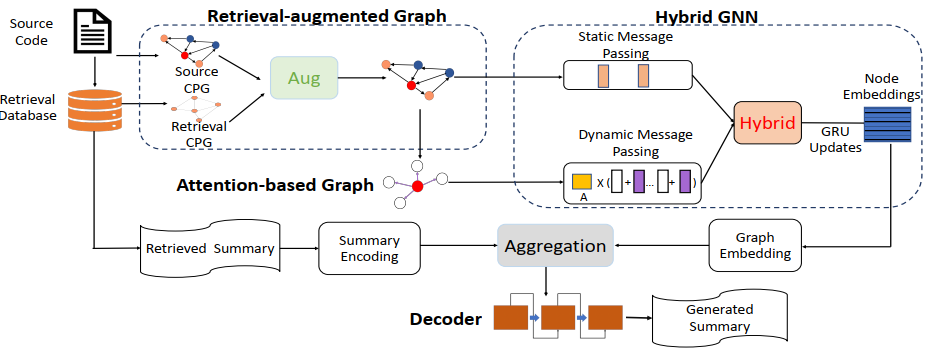
\includegraphics[width=.8\textwidth]{pics/HGNN.png}
	\label{fig:hgnn}
	\caption{Overview of HGNN}
\end{figure}

论文提出的方法是Hybrid GNN(Fig.\ref{fig:hgnn}),首先根据代码的抽象语法树表示成Graph(Fig.\ref{fig:cpg}),再从代码数据集中找到与当前代码最相似的代码(除去当前的函数)及对应的summarization,当前代码的Graph经过最相似的代码的Graph增强后得到static graph,经过注意力机制后生成dynamic graph,在static/dynamic graph上进行message passing,再通过Hybrid massage passing(即将同一个结点在static和dynamic graph中的表征融合后再进行massage passing)。除此之外,还会利用找到的最相似的代码的summarization的表征,将最终得到的结点表征与summarization表征进行拼接后输入基于注意力的LSTM,得到目标代码的表征。

\begin{figure}[h]
	\centering
	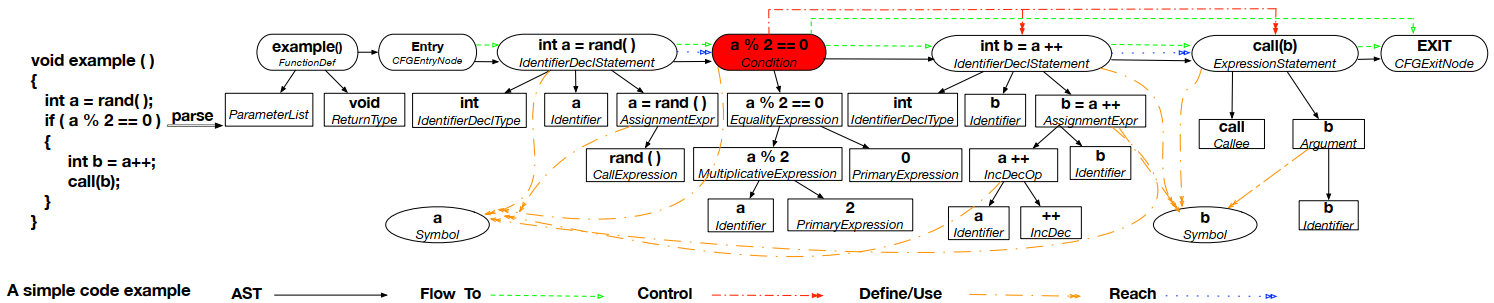
\includegraphics[width=.8\textwidth]{pics/CPG.png}
	\label{fig:cpg}
	\caption{An Example of Code Property Graph(CPG)}
\end{figure}

